\documentclass{UoYCSproject}
\addbibresource{REFERENCES.bib}

\BEng

\supervisor{Dr. Christopher Crispin-Bailey}

\begin{document}

\title{Generation of Hardware Accelerators for the Microblaze Soft Processor}
\author{Jay Valentine}

\maketitle

\begin{abstract}
\end{abstract}

\chapter{Introduction}

\section{Motivation}

\chapter{Literature Review}

\section{Moore's Law and Dennard Scaling}

In 1965, Gordon Moore predicted that the number of transistors in an integrated circuit will double
approximately every two years  \cite{moore}. Similarly, Dennard scaling describes the way in which transistor power density
remains constant as the transistors themselves shrink in size \cite{dennard}. These phenomena combined allow for exponential
transistor-density increases, and this has been exploited to produce exponentially higher performance in
microprocessors year on year.

\begin{figure}[h]
\center{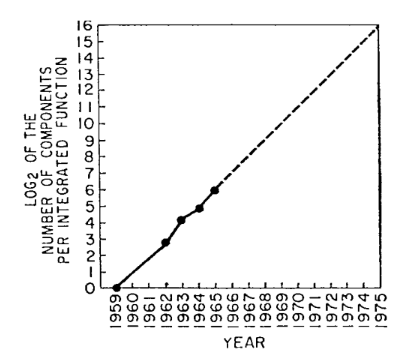
\includegraphics[width=\textwidth]
{figures/moore.png}}
\caption{Moore's 1965 prediction. \cite{moore}}
\end{figure}

However, in more recent times, a breakdown in this scaling has been observed. In the past, Dennard scaling has allowed
microprocessor manufacturers to offset the increased energy cost of faster transistor switching, resulting in higher
and higher clock speeds. However, more recently, microprocessor clock speeds have remained relatively static. This is
due to a breakdown in Dennard scaling for very small transistors, and has caused microprocessor manufacturers to instead
pursue increased performance by the use of multicore designs.

\begin{figure}[h]
\center{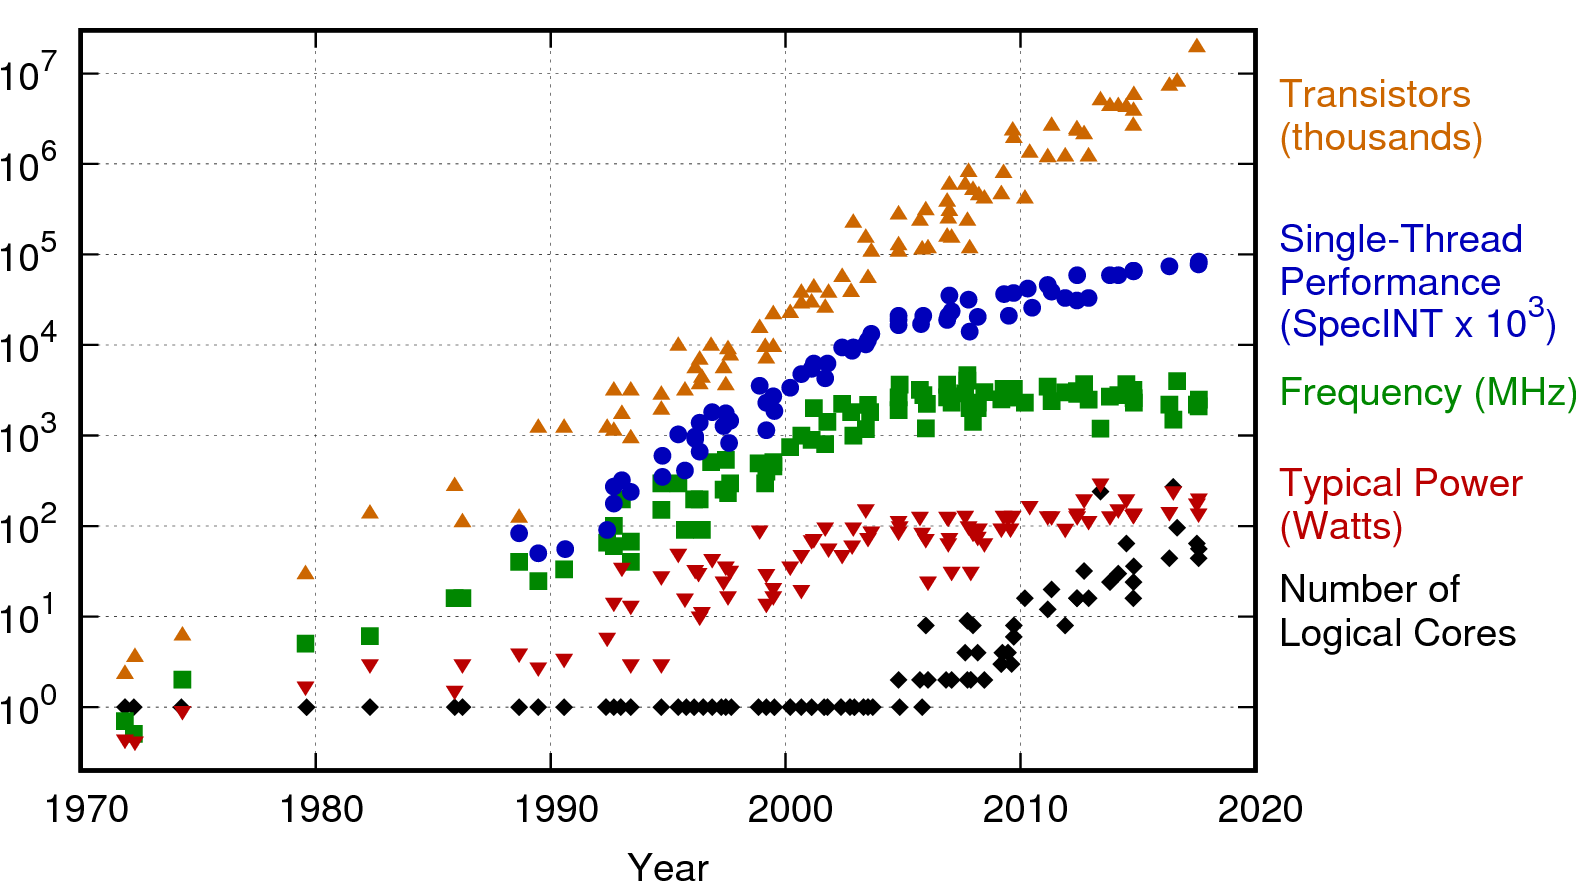
\includegraphics[width=\textwidth]
{figures/cpu-speed.png}}
\caption{Trends in microprocessors since 1970. \cite{karlrupp}}
\end{figure}

\section{Dark Silicon}

Dark silicon is a phenomenon which has been observed as transistor density in microprocessors has increased.
It occurs as issues relating to energy efficiency and transistor utilization lead to a gap between the
observed speedup and that predicted by extrapolating from historic performance gains.
In \cite{darksilicon}, it is predicted that with 22nm transistors, 21\% of the chip will be dark silicon,
with this rising to 50\% at 8nm. This prediction shows that dark silicon will become a serious limitation
as transistor density grows, especially in areas where energy efficiency is a primary concern.

Dark silicon also becomes a limiting factor with manycore devices. Even when energy consumption is not a
concern, the limited parallelism of most applications results in a dark silicon gap when running with
manycore devices. Again, \cite{darksilicon} shows that beyond a certain number of cores the speedup achieved
is negligible. This is another kind of dark silicon - the underutilization in this case is not a result of
energy concerns but is caused by the limited parallelism of the application being unable to exploit all of
the cores of a device.

There have been several broad responses to this phenomenon.
In \cite{four-horsemen}, Taylor gives two pessimistic predictions regarding the future of silicon
utilization. The first, the 'shrinking horseman', predicts that chips will begin to shrink as a result of
the utilization wall. This would lead to an increase in cost per mm\textsuperscript{2} of silicon, as
design costs, test costs, marketing costs, etc. Put simply, "exponentially smaller chips are not
exponentially smaller".

The second, perhaps slightly less pessimistic, prediction in Taylor's paper
is referred to as 'the dim horseman', and describes the under-clocking or infrequent use of
general-purpose silicon in order to meet power budgets. While a better alternative than the shrinking
of chips, this still causes issues as the chip is no longer operating at maximum capacity.
Taylor outlines several options for the use of this 'dim silicon'. The first, and perhaps most obvious,
is the use of homogenous architectures, but with some cores operating at a lower clock speed, or
even being turned off intermittently. However, there are other 'dim silicon' approaches that make better
use of the unutilized silicon area. One approach is to increase cache sizes, as cache memory is less
power-dense than a processing core would be. This has a secondary benefit as well, in that a larger
cache will reduce the number of cache misses, thereby decreasing the number of power-hungry off-chip
accesses.

Finally, Taylor also describes 'the specialized horseman'. This approach is to use the dark silicon area
not for general-purpose computing, but for a large number of specialized cores, which would be much
faster or energy efficient than a general-purpose core, allowing for increased energy efficiency at the
cost of silicon area.

\section{Energy Efficiency}

Many attempts at managing dark silicon for energy efficiency have been made. One approach, outlined in the
GreenDroid project \cite{greendroid}, is to replace areas of a chip that cannot be utilized due to dark
silicon with specialized cores, designed to perform common computations. In the GreenDroid architecture,
these cores account for over 90\% of execution time, leading to a significant reduction in energy
consumption. This was aided by profiling of the Android platform, allowing the identification of 'hot'
(frequently-executed) portions of code to be offloaded to specialized logic. It was found that Android,
due to the organization of its components, was an ideal candidate for this approach.

The first step in the GreenDroid toolchain is the profiling of the target application, in this case the
Android OS stack, to identify 'hot' functions or loops. Each 'hot-spot' is then translated into a c-core,
with instructions being grouped together by basic block and control flow through the function/loop being
tracked by a state machine.

A similar approach is taken by Arnone in \cite{arnone-thesis}. Here, Arnone outlines a method of
generating accelerator cores for a stack architecture, resulting in both timing
and power improvements. Two architectures for generated cores are described: composite and wave-core.
Composite cores are simple state machines with instructions mapped to states. Composite cores attempt to
optimise for logic area by reusing existing logic between states. Conversely, the wave-core
architecture avoids the reuse of logic between states, reducing power density at the cost of increased
logic area (due to potentially duplicated functionality). In both cases the resulting accelerator core is
more energy-efficient than the general-purpose processor is at the same task.

\section{Performance}

In \cite{high-performance-microarchitecture}, Razdan and Smith attempt to simplify the state machine model
to reduce synchronization complexities. They developed a toolchain which was able to extract instruction
streams that could be 'outsourced' to an accelerator core after code generation. These cores are not state
machines but are instead streams of instructions translated into hardware, such that a previously
multi-cycle operation can be executed in a single cycle. The instruction stream that existed in the
original application can then be replaced by a single instruction, \textit{expfu}, which triggers
the respective accelerator core and retrieves the result. As SoCs (as opposed to discrete units) become
more prevelant, this work shows that there may be a place for FPGAs in such a system.

Similar work has been done with GARP \cite{garp}, in which an FPGA and a MIPS processor are combined on the
same die, with the intention that certain portions of an application could utilize the reconfigurable
hardware to achieve performance increases. The paper acknowledges the difficulties with reconfigurable
computing - as configuration time is too expensive for limited-use configurations, and "in real programs,
much code is not repeated often enough to be worth loading into an FPGA". GARP attempts to circumvent this
limitation by the use of a hybrid architecture, and by providing mechanisms by which the reconfigurable
hardware can be used by applications to speed up repeated blocks functionality, with the rest of the
application executing on the MIPS core.

\printbibliography

\end{document}